\documentclass{article}

\usepackage[margin = 2.5 cm]{geometry}
\usepackage[utf8x]{inputenc}
\usepackage{graphicx}
\usepackage[magyar]{babel}
\usepackage{amsmath}
\usepackage{booktabs}
\usepackage{mathrsfs}
\usepackage{float}
\usepackage{multirow}
 

\begin{document}
	\begin{titlepage}	
		%címlap
		\vspace*{5 cm}
		\begin{center}
			\Huge \textbf{Tárgymanipuláció kulcspontok detektálásán alapuló képfeldolgozással}
			\LARGE
			
			Szakmai gyakorlat beszámoló\\
			\vspace{12pt} \normalsize
			Ayhan Dániel\\
			LIIAE1
		\end{center}
		\vspace{6 cm}
		Témavezető:\\
		\\		
		Dr. Kiss Bálint
		\begin{center}		
			\vfill
			Budapest, \today	
		\end{center}
	\end{titlepage}
	\newpage
	
	\thispagestyle{empty}
	\tableofcontents
	
	\setlength{\parindent}{0 em}	
	\setlength{\parskip}{1em}
	
	\newpage
	\setcounter{page}{1}
	\section{Bevezetés, feladatkitűzés}
	A szakmai gyakorlatomat a Budapesti Műszaki és Gazdaságtudományi Egyetem Irányítástechnika és Informatika Tanszékén végeztem. A feladat egy tetszőleges tárgy lokalizálása volt képfeldolgozás segítségével. Lokalizálás alatt a tárgy pontos pozícióját és orientációját, azaz \textit{helyzetét} értem. A tárgyról előzetesen bármilyen információnk lehet, célszerű erre az adathalmazra is képfeldolgozással szert tenni. 
	
	A választott módszer a következő volt: a tárgyról készült képen keressünk \textit{kulcspontokat}, majd ezekhez generáljunk \textit{leíróvektort}, amely a lehető legtöbb fajta torzításra invariáns. Ezeket a vektorokat két különböző helyzetből készült képen össze lehet párosítani. A kamera helyzetének ismeretében különböző módszerekkel ezekből a párosításokból 3D koordinátákat lehet kapni. Így olyan adathalmazhoz jutottunk, amelyben leíróvektorokhoz (vagy röviden: leírókhoz) 3D koordinátákat rendeltünk. Ezek után a tárgyról egy ismeretlen helyzetből készült képen ugyanezeket a kulcspontokat megkereshetjük. A megtalált kulcspontokhoz számíthatunk leírókat, amelyeket összepárosítva az adathalmaz leíróival megkaphatjuk a képen talált kulcspontok 3D koordinátáit. Innen a megfelelő algoritmussal kiszámolhatjuk a kamera külső paramétereit, azaz az objektumhoz képesti helyzetét. Ezzel meghatároztuk az objektum helyzetét a kamera koordináta-rendszerében.
	
	\section{A gépi látás alapfogalmai}
	Az algoritmusok áttekintése előtt ismerkedjünk meg a gépi látásban, képfeldolgozásban használatos fogalmakkal. A kamerát úgynevezett pinhole-kameramodellel írjuk le. Ez a modell azt feltételezi, hogy a kép keletkezése olyan módon történik, hogy a háromdimenziós teret perspektivikusan vetítjük a képsíkra.

%\begin{figure}[H]
%\centering
%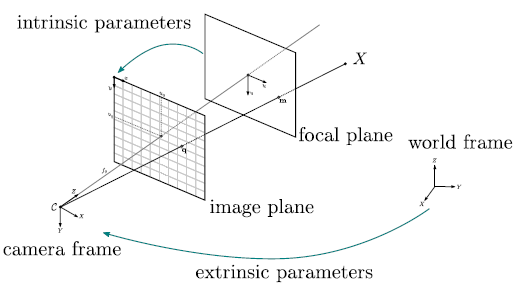
\includegraphics[width=0.7\linewidth]{image3.png}
%
%\caption{A pinhole-kameramodell. Forrás: http://openmvg.readthedocs.io/}
%\end{figure}
	
	
A kamerához definiálható egy kamera koordináta-rendszer. Ennek a koordináta-rendszernek az origójának a vetítés középpontját tekintjük, a z tengelye merőleges a vetítés síkjára. A kép koordináta-rendszer síkbeli koordináta-rendszer, a síkra vetített pontokat értelmezzük ebben. x és y tengelyei a kamera koordináta-rendszer tengelyeivel egyirányúak. Amennyiben homogén koordinátákkal jellemezzük a tér pontjait, mind a perspektív vetítés, mind a világ koordináta-rendszer és a kamera koordináta-rendszer közötti eltolás, forgatás mátrixszal kifejezhető: 

\begin{equation}
w\left[
\begin{array}{c}
u \\ v \\ 1
\end{array}
\right] = \left[ 
\begin{array}{ccc}
f_x & \gamma & u_0 \\
0 & f_y & v_0 \\
0 & 0 & 1
\end{array}
\right]\left[
\begin{array}{cccc}
r_{11} & r_{12} & r_{13} & t_1 \\
r_{21} & r_{22} & r_{23} & t_2 \\
r_{31} & r_{23} & r_{33} & t_3 \\
\end{array}
\right]\left[
\begin{array}{c}
x \\ y \\ z \\ 1
\end{array}
\right]
\end{equation}
 
A vetítés mátrixát kameramátrixnak hívjuk, a paramétereit pedig a kamera belső paramétereinek nevezzük. Mivel ezek a kamera rendeltetésszerű használata során nem változnak jelentősen, a kamera szerves részei, egyszeri kalibrálással meghatározhatók. A koordináta-rendszerek közti transzformáció paraméterei a külső paraméterek. Az összes paraméter meghatározható kellően nagy számú pontpár segítségével. A pontpárok alatt a világ koordináta-rendszerben ismert pozíciójú pontokat és azok kép koordináta-rendszerben megadott vetületét értjük.

A kameramátrixot a feladat megoldása során ismertnek feltételeztem, hiszen az időben állandónak tekinthető.

A valóságban a pinhole kameramodell sajnos nem állja meg a helyét, a képet többféle torzítás terheli például abból adódóan, hogy nem vetítést alkalmazunk, hanem lencserendszert, valamint, hogy a detektoron elhelyezkedő pixelek gyártástechnológiája nem tökéletes. ezeket a paramétereket most elhanyagoljuk, így a fenti összefüggésben a $\gamma$ paraméter 0 lesz.

		
	\newpage
	\section{Kulcspontkereső algoritmusok}
	
	A kulcspontkereső algoritmusok célja olyan pontok megtalálása a képen, amelyek valamely környezete vizuálisan érdekes, jól elkülöníthető, egyedi. Céljuk továbbá, hogy ezekhez a pontokhoz olyan jellemző mennyiséget rendeljenek, amely alapján az adott pont egy másik képen is megtalálható, és ugyanazt a jellemző mennyiséget eredményezi. Ezzel a mennyiséggel szemben támasztott követelmény az is, hogy legyen invariáns minél többféle képalkotáskor előforduló transzformációra, mint például a skálázás, elforgatás. A jellemző mennyiség a legtöbb algoritmus esetében egy tulajdonság-leíró vektor, vagy leíróvektor, röviden csak leíró.
	
	\subsection{SIFT kulcspontkeresés}
	
	A SIFT (Scale Invariant Feature Transform) egy kulcspontkereső algoritmus. Az általa generált leíró egy 128-elemű vektor, amely invariáns eltolásra, elforgatásra, skálázásra, a megvilágítás kismértékű megváltozására, zajra, és a kamera pozíciójának kismértékű megváltozására. Nem invariáns a projektív transzformációra, tehát a kamera helyzetének jelentős megváltozására.
	
	Az algoritmus főbb lépései a következők:
	
	\begin{enumerate}
	\item Kulcspont-jelöltek skálainvariáns detektálása
	\item Szubpixeles lokalizáció
	\item Kulcspont-jelöltek szűrése
	\item Jellemző orientáció meghatározása
	\item Lokális orientáció-hisztogramok számítása
	\item Leíró-generálás
	\end{enumerate}
	
	\subsubsection{Kulcspont-jelöltek skálainvariáns detektálása}
	Az algoritmus első lépéseként a képen érdekesnek tűnő pontokat keresünk. Ezt DoG (Difference of Gaussians) szűrőkkel érjük el. A DoG szűrő a képet különböző mértékű (szórású) Gauss-szűrésnek veti alá, majd ezek különbségét veszi. Így az élkiemeléshez hasonló képet kapunk, ám legjobban a szórás méretébe eső térfrekvenciájú részletek kerülnek kiemelésre. A szűrést különböző szórású kernelekkel elvégezve különböző mérettartományokba eső képrészleteket emelhetünk ki. Az így kapott képeken megtalált szélsőértékeket tekintjük kulcspont-jelöltnek.
	
	\subsubsection{Szubpixeles lokalizáció}
	A kulcspontok szubpixeles lokalizációjához az egyes dimenziókban (x, y, skála) másodfokú közelítést alkalmazunk, és így keressük meg a valódi szélsőérték helyét pixel alatti és skálafaktornál nagyobb pontossággal.
	
	\subsubsection{Kulcspont-jelöltek szűrése}
	Az algoritmus ezen a pontján sok olyan pontot is megjelölt, amelynek képi helyzete nem egyértelmű, pl. egy homogén régiót, vagy élt jellemeznek a képen nem pedig egy pontot. Ezek kerülnek kiszűrésre ebben a lépésben. A szűrés során az adott pontban kiszámoljuk a másodfokú deriváltakból álló Hesse-mátrixot. Ennek a mátrixnak a sajátértékei szolgálnak információval a pont környezetéről. Amennyiben mindkét sajátérték kicsi, a pont környezete homogén. Ha az egyik kicsi, a másik pedig nagy, élszerű pontról beszélhetünk. A "kicsi" és "nagy" fogalmak természetesen kvalitatívak, a számszerű értékek tapasztalati úton kerülnek meghatározásra, az algoritmus bemeneti paraméterei. Ezeket az élszerű és homogén környezetű pontokat ezen a ponton eldobjuk.
	
	\subsubsection{Jellemző orientáció meghatározása}
	Az orientációhoz hisztogramot használunk, amelynek 36 osztálya van, mindegyik 10°-ot fed le. A kulcspont környezetében minden pontban kiszámítjuk a gradiensvektort, majd ennek irányának megfelelően a hisztogram adott osztályába tesszük. A maximális orientációt másodfokú interpolációnak alávetve határozzuk meg a jellemző orientációt. Amennyiben több kiugróan nagy orientáció van a hisztogramban, a kulcspontot lemásoljuk, és mindegyik orientációval újat hozunk létre. Így érjük el az elforgatás-invarianciát.
	
	\subsubsection{Lokális orientáció-hisztogramok számítása}
	A képpont 16x16 pixeles környezetét felosztjuk 4x4 darab 4x4-es blokkra. Minden blokkhoz létrehozunk egy 8-osztályos orientáció-hisztogramot, amibe az adott pixeleknek az előző lépésben meghatározott orientációhoz képesti relatív gradiens-iránya kerül.
	
	\subsubsection{Leíró-generálás}
	A leíró-vektor elemeit az előző lépésben kiszámolt hisztogram osztályainak gyakoriságai adják. A 4x4 darab 8-osztályos hisztogramból így 128-elemű vektort kapunk. Ezt a vektort megvilágítás-invariancia céljából normalizáljuk.
	
	\subsection{SURF kulcspont-keresés}
	A SURF (Speeded Up Robust Features) algoritmus hasonló elven működik, mint a SIFT, ám az egyes lépésekhez különböző megoldásokat alkalmaz. A kulcspont-jelöltek keresésénél a Gauss-szűrést ún. box-filterrel közelíti, amit az integrális képből számol. Az integrális kép $(x,y)$ koordinátájú pixele azon pixelek összegét tartalmazza, amik egy megadott téglalapon belül találhatók. E téglalap bal felső sarka a kép bal felső sarkával esik egybe, a jobb alsó pedig az $(x,y)$ pixel. Érdekes pontoknak azokat fogja venni, ahol a Hesse-mátrix determinánsa lokálisan maximális. Itt is a pontosság érdekében interpoláljuk a megoldást. Az orientáció meghatározásnál egy adott Euklideszi norma szerinti (kör alakú) környezeten belül található pontok (Haar-wavelet válaszával közelített) gradiens-irányát veszi figyelembe, és egy csúszóablakkal történő kereséssel határozza meg a domináns orientációt. A leíró-generálásnál a kulcspont környezetét 4x4-es blokkokra osztja, és ezekhez a blokkokhoz rendel egy négyelemű vektort, amit a gradiensek alapján számít. Így 4x4x4, azaz 64-elemű leíróvektort kapunk.
	
	\newpage
	\section{Leíró-párosító algoritmusok, párosítás-szűrések}
	Miután a kulcspontdetektáló algoritmus megkereste a képen az érdekes pontokat, leíró-vektort generált hozzájuk. Ezt két különböző képen elvégezve az így kapott leírókat párosítanunk kell, ha megfeleltetéseket akarunk a kulcspontok között találni. Mivel a leírók  n-dimenziós vektorok, ezért két leíró közötti hasonlóságot egyszerűen lehet számszerűsíteni, pl. a különbségük L2 normájával. A probléma abból fakad, hogy nagyméretű képeken sok (1000-es nagyságrendű) leírónk van, és ezeket kell másik, hasonló méretű leíró-halmazhoz párosítani.
	
	A legegyszerűbb megoldás a brute force módszer, vagyis mindegyiket mindegyikkel összehasonlítjuk. Ez lassú ugyan, de garantáltan a legjobb megoldást adja. Egy másik megoldás a FLANN (Fast Library for Approximate Nearest Neighbors) algoritmus, ami gyors, de csak közelítő megoldást ad.
	
	Az algoritmusok garantáltan sok hibás párosítást is eredményeznek, ezeket feltétlenül szűrni kell, amelyekre több módszer is van, a következőkben ezeket mutatom be. Mindegyik algoritmusban egy $d$ vektorhoz keresünk párt a $B$ halmazból, ahol $d$ az egyik képen megtalált leírók közül egy, $B$ pedig a másik képen megtalált leírók halmaza.
	
	\subsection{Arányteszt alapú párosítás-szűrés}
	Ez a heurisztikus módszer azon a feltételezésen alapul, hogy a helyes párosítás esetén $d$ sokkal közelebb van a párjához, mint más vektorokhoz. Amennyiben egy hamis párosítást veszünk, $d$ vektorhoz a legközelebb eső $B$-beli vektor valószínűleg nem lesz $d$-hez sokkal közelebb, mint a második legközelebbi, hiszen a hamis párosításnál a legjobb megoldás nem sokkal jobb a második legjobbnál.
	
	Éppen ezért ez a szűrés azokat a párosításokat tartja meg, amelyeknél a legjobb megtalált $B$-beli vektor ($b_{true}$) és a második legjobb vektor ($b_{false}$) közötti távolságok aránya nagy:
	\begin{equation}
	\frac{\|d-b_{true}\|}{\|d-b_{false}\|}\ll 1
	\end{equation}
	
	A gyakorlatban az aránynak a küszöbértékét $0,6..0,8$ közé szokás venni.
	
	\subsection{Kereszt-ellenőrzéses szűrés}
	Ez a módszer azt a feltételezést használja, hogy ha $d$ és $e$ párok a két képen, akkor nincs olyan más vektor $e$-n kívül az ő halmazában, ami $d$-hez közelebb lenne, viszont $e$-hez sem találni $d$-nél közelebb lévő vektort. Ez a szűrés akkor fogadja el a párt, ha $d$-hez $e$ van legközelebb a második képen talált leírók közül, $e$-hez pedig $d$ az első képen lévők közül.
	
	\subsection{Epipoláris egyenes használata}
	Amennyiben ismerjük a két képhez tartozó kamerapozíciót, minden ponthoz az első képen definiálható egy egyenes a második képen, amely egyenes mentén a pont párja elhelyezkedhet. Ezt hívjuk epipoláris egyenesnek. Ennek az információnak a birtokában a párosításnál vehetjük eleve csak az epipoláris egyenesre illeszkedő pontokat, és azokhoz párosítjuk a $d$ leírót, vagy a párosítás után eldobhatjuk azokat a párokat, ahol a megtalált kulcspont nem illeszkedik az egyenesre, így kevesebb párt kapunk majd.
	
	\subsection{Homográfia-alapú szűrés}
	A homográfia olyan transzformáció, ami egy síkbeli alakzat pontjaihoz tartozó képi pontok között teremt kapcsolatot. Segítségével az egyik képen található pont másik képen való pozícióját lehet meghatározni. A homográfia jól párosított pontok segítségével meghatározható. A hibás párosításokat RANSAC algoritmussal kiszűrhetjük, amikor a párosításokra homográfiát illesztünk, így az algoritmus nagy mennyiségű hibás adat esetén is jól működik. Ez a módszer csak sík objektumokra használható.
	
	\section{3D rekonstrukció}
	A 3D rekonstrukció során egy térbeli objektum pontjainak koordinátáit kívánjuk meghatározni. Ez esetünkben különböző nézőpontból készült képek alapján történik. A problémát megoldó algoritmusokat Structure from Motion (SfM), vagy Multi-View Stereo (MVS) algoritmusoknak hívjuk. Amennyiben a kamera külső paraméterei ismertek, a probléma lineáris legkisebb négyzetek módszerével megoldható. A külső paraméterek hiányában a feladat nemlineáris legkisebb négyzetek problémává alakítható, amelyet célszerű Levenberg-Marquardt algoritmussal megoldani. Ennek a nemlineáris problémának a megoldása a szakirodalomban \textit{bundle adjustment} néven található meg. Ezzel most nem foglalkozunk, ugyanis számunkra ismertek a kamera külső paraméterei.
	
	A 3D rekonstrukció kimenete általában egy pontfelhő. Amennyiben csak kulcspontok párosítását használjuk, és azok térbeli helyzetét határozzuk meg, ún. ritka pontfelhőt kapunk. Ha teljes 3D-s modellt akarunk kapni, vagy a teljes megfigyelt környezetet vissza akarjuk állítani, akkor sűrű pontfelhőre van szükségünk. Számunkra a ritka pontfelhő is elegendő.
	
	A pontok térbeli pozíciójának meghatározása háromszögeléssel történik. A probléma precíz megfogalmazása a következő: Adott $n$ pont ismert térbeli helyzetű kamerák által készített képeken. Keressük azt a 3D-s tárgypontot, amelyet a kamerák képsíkjaira visszavetítve az eredeti pontoktól való távolságok négyzetösszege minimális.

	\subsection{Leíró-párosító algoritmusok sajátosságaiból adódó problémák}
	A feladat bonyolultsága fokozható, ha figyelembe vesszük, hogy a párosító algoritmusok téves párosításokat is tartalmaznak, valamint, hogy egy leíróhoz lehet, hogy csak kevés (egy vagy kettő) másikat sikerül párosítani még több kép esetén is.
	
	A párosításokat értelmezhetjük ritka erdő gráfként, ahol a csúcsok a kulcspontok, és azok leírói, az élek pedig a párosításokat jelentik. Értelemszerűen ha feltételezzük, hogy minden párosítás helyes, akkor minden fa (azaz egybefüggő részgráf) egy-egy tárgyponthoz tartozó leírókat tartalmaz. 
	
	A tesztek alapján, amiket végeztem, azt lehet mondani, hogy 5 tesztkép esetén mindegyiket mindegyikkel párosítva a csomópontok több, mint feléből csak egyetlen él fut ki, azaz a hozzájuk tartozó leírókhoz a többi 4 képből csak egyen sikerült párt találni. A tesztek azt támasztják tehát alá, hogy a gráf kellően ritka.
	
	\subsubsection{A ritkaság korrigálása}
	\label{extension_doc}
	A gráf sűrítése érdekében megtehetjük azt, hogy pl vesszük az összes olyan csúcs-hármast, amelyik majdnem teljes algráfot (kvázi-klikket) alkot, vagyis a 3 élből csak egy hiányzik, és teljessé tesszük, bízva abban, hogy a párosító algoritmus valamilyen oknál fogva a behúzott élnek megfelelő párosítást nem találta helyesnek, pedig az. Ezt megtehetjük bármilyen csúcs-$n$-esre is.
	
	\subsubsection{Téves párosítások szűrése}
	A téves párosítások figyelembe vételéhez érdemes RANSAC elven működő algoritmust alkalmazni, vagyis kevés, feltehetőleg helyes adatból számolni az eredményt, majd ehhez a közelítő megoldáshoz hozzávenni az ezzel konzisztens adatokat, és téves adatnak minősíteni az inkonzisztens adatokat. Jelen esetben ez jelentheti például azt, hogy ha veszünk egy fához tartozó csúcsokat, két véletlenszerűen kiválasztott csúcs alapján háromszögeléssel kiszámítjuk a 3D pozíciót, majd megnézzük, hogy a pontot a képekre visszavetítve mekkora eltérést kapunk a fa többi csúcsában tárolt pozíciókhoz képest. Amennyiben kis eltérést kapunk, az adott csomópontot helyes adatnak tekinthetjük. Végül az összes helyes adat felhasználásával egy pontosabb pozíciót számolhatunk háromszögeléssel.
	
	\section{Külső paraméterek meghatározása, PnP probléma}
	Az előző fejezetekben leírt módszerekkel létrehozhatunk egy adathalmazt, amelyben leíróvektorokhoz tartozó tárgypontok 3D koordinátáit tároljuk. Ennek segítségével tudjuk egy ismeretlen pozícióból készült kép külső paramétereit meghatározni. Ehhez nem kell mást tennünk, mint ugyanazt a kulcspontdetektáló és leírógeneráló algoritmust végigfuttatni a képen, mint amit az adathalmaz generálásakor használtunk, majd az így kapott kulcspontokat a leírók segítségével az adathalmazban található leírókhoz párosítani. Ezzel olyan megfeleltetésekhez jutottunk, amelyek a tesztképen lévő pontokhoz rendel 3D koordinátát.
	
	Azt a feladatot, amely ismert térbeli helyzetű tárgypontok és a hozzájuk tartozó képi pontok alapján próbálja meghatározni a kamera külső paramétereit PnP, azaz Perspective-n-Point problémának nevezzük. 
	
Ennek egyik verziója a P3P algoritmus, amely csak 4 pontpárból számítja a paramétereket. Három pont kell ahhoz, hogy véges sok egyértelműen megoldást kapjunk (négy ponttal már túlhatározott lenne a feladat). A negyedik pontot az algoritmus arra használja fel, hogy a véges sok megoldás közül kiválassza a helyeset. Ezt úgy teszi meg, hogy a lehetséges négyféle megoldás közül azt választja, amelyikkel a negyedik pontot a képre vetítve a legkisebb hibát kapjuk a megadott képi ponthoz képest. Ezt aztán tetszőleges optimumkereséssel tovább lehet finomítani, pl. Levenberg-Marquardt eljárással. Ezt az eljárást használhatjuk akkor is, ha több, mint négy pont áll rendelkezése.
	
	\section{Megvalósítás}

	Az ismertetett algoritmusok mind implementálva vannak az OpenCV függvénykönyvtárban. Ennek a Python nyelvhez készült burkolóját használtam.
	
	Amennyiben az adathalmaz, vagyis a tanítóképeken megtalált kulcspontok, leírók és tárgypont-koordináták közti megfeleltetések rendelkezésre állnak, a tesztkép külső paramétereit egyszerű meghatározni. Ehhez az OpenCV beépített SolvePnPRansac függvényét használtam. Ez az algoritmus a PnP probléma megoldását számolja ki, és mivel RANSAC módszert alkalmaz, ezért a nagy arányú hibás adatra is robusztusan működik.
	
	A megvalósítás legfőbb kérdése az adathalmaz létrehozásának mikéntje. Az algoritmus főbb lépései a következők:
	
	\begin{enumerate}
	\item Tanítóképek készítése
	\item A tanítóképek külső paramétereinek meghatározása
	\item A képeken kulcspontok keresése, leírók generálása
	\item A leírók párosítása képpáronként, szűrés
	\item A párosítások kiegészítése
	\item A 3D pozíciók meghatározása
	\end{enumerate}
	
	A következő alfejezetekben az egyes lépésekhez használt módszereket mutatom be.
	\subsection{Tanítóképek készítése}
	A fejlesztés során 5 tanítóképet használtam. Mindegyiken egy távirányító volt látható, alatta pedig egy kalibráláshoz használt marker. A távirányító azért volt jó választás, mert kulcspontokban gazdag, sok felismerhető jellemző van rajta. Egy ilyen képet láthatunk alább:
	
%	\begin{figure}[H]
%\centering
%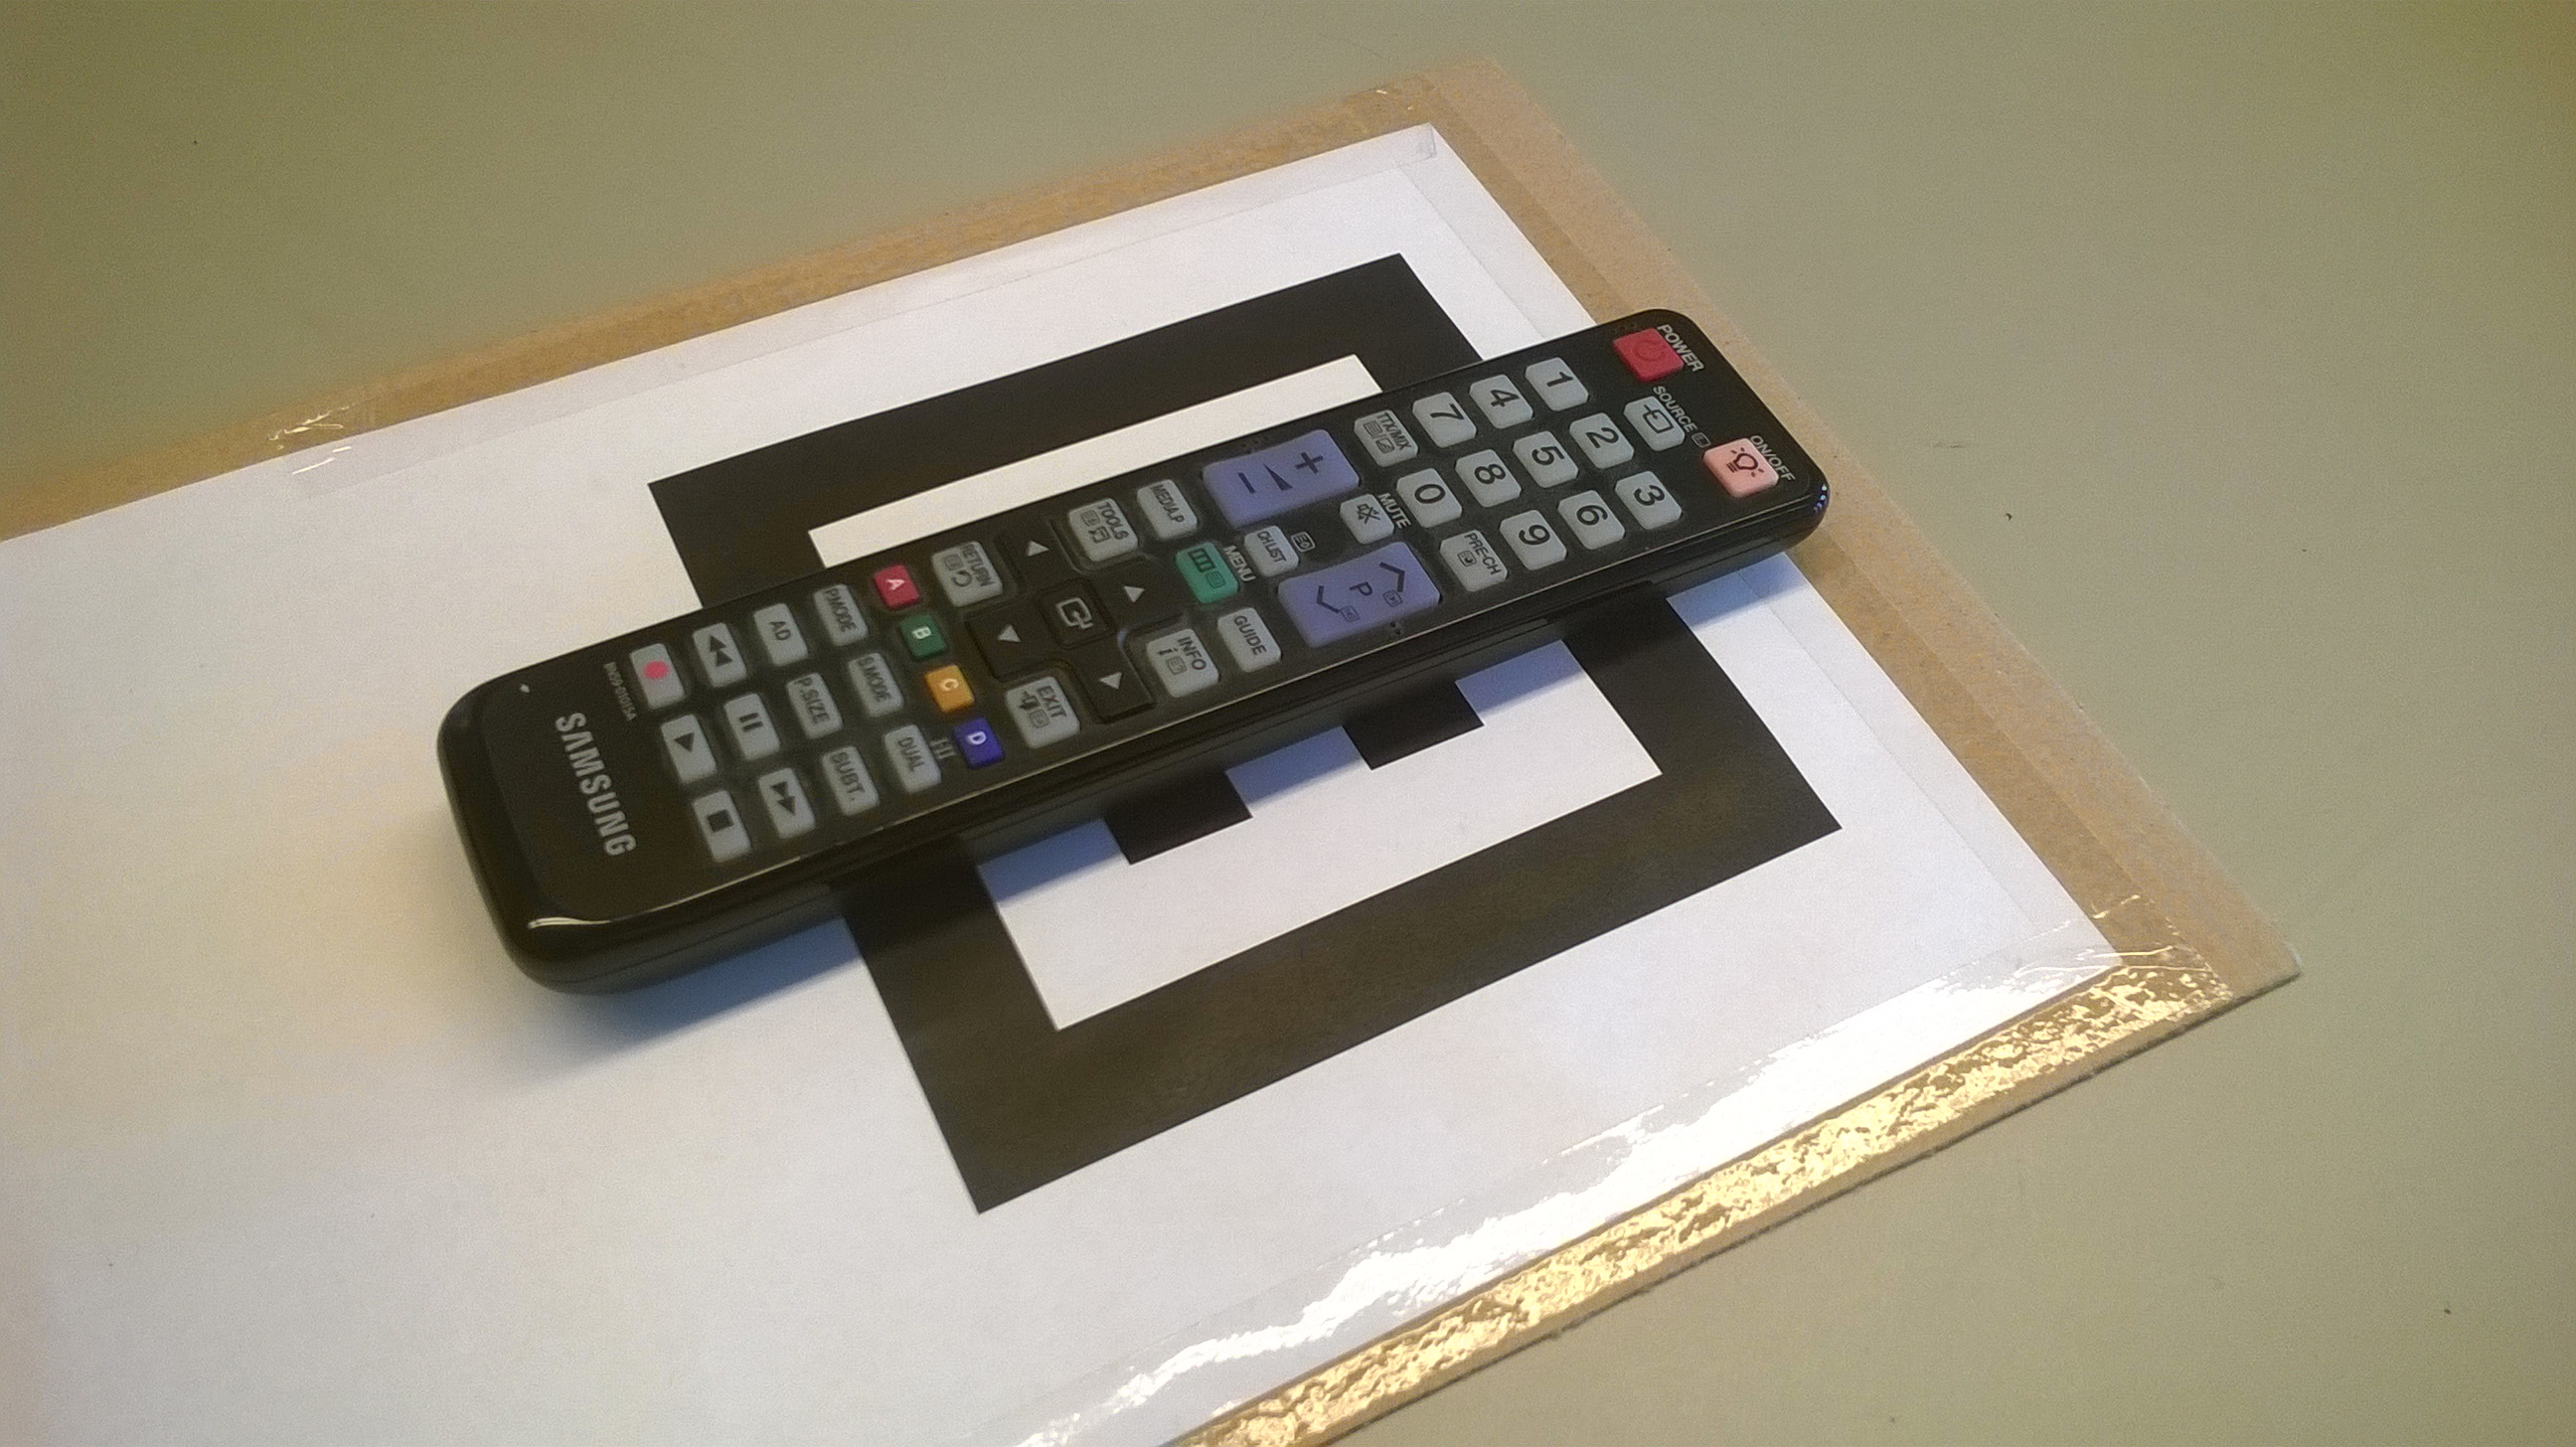
\includegraphics[width=0.7\linewidth]{006.jpg}
%\end{figure}
	
	\subsection{Külső paraméterek meghatározása}
	A kamera helyzetének meghatározása a képen látható marker segítségével történik. Jelenleg ez teljesen manuális.
	
	\subsection{Kulcspontkeresés, leírógenerálás}	
	A kulcspontkereséshez SURF algoritmust használok. Ez gyorsabb a SIFT algoritmusnál, kisebb leírót generál, és valamivel robusztusabb bizonyos esetekben.
	
	\subsection{Leíró-párosítás, szűrés}
	A leíró-párosításnál többféle módszert is kipróbáltam.
	
	\subsubsection{Párosítás epipoláris egyenesekkel}
	\label{epilines}
	Ennél a módszernél a párosítás során az adott kulcspont párját csak a másik képen behúzott epipoláris egyenes mentén keressük. a keresés brute force módszerrel történik. A párosítást a másik irányba is lefuttatjuk, és kereszt-ellenőrzéses szűrésnek vetjük alá.
	
	\subsubsection{Párosítás epipoláris egyenesekkel több kulcsponthoz}
	\label{epilines_multiple}
	Ez a módszer annyiban különbözik az előzőtől, hogy nem csak a legjobb párosítást tartjuk meg, hanem a legjobb $n$ darabot. A tesztelés során $n=4$-et használtam.
	
	\subsubsection{Párosítás epipoláris egyenesekkel és homográfiás szűréssel}
	\label{epilines_homogr}
	A módszer ugyanaz, mint a \ref{epilines} részben ismertetett, de a végén lefuttatunk egy homográfia-alapú szűrést.
	
	\subsection{A párosítások kiegészítése}
	\label{extension}
	A gráf kiegészítéséhez az \eqref{extension_doc} részben ismertetett módszert használtam csúcs-hármasokra. Ezt az algoritmust kétszer futtattam egymás után.
	
	\subsection{3D koordináták meghatározása}
	\subsubsection{Klikkalapú rekonstrukció}
	\label{clique_pos_simple}
	Ennél a módszernél a párosítási gráfban megtalált klikkeket (teljes részgráfokat) veszem figyelembe. Feltételezem, hogy a klikkek minden éle helyes párosítás, és így a klikk csúcsaiból számítom a 3D pozíciót többnézetes háromszögeléssel. Megadható egy-egy küszöbérték a visszavetítési hiba átlagos és maximális értékére, ha ezt túllépi a hiba, a klikket eldobjuk, és nem számítunk hozzá 3D pozíciót. Az algoritmust 3-as klikkekre futtattam.
	
	\subsubsection{Egyszerű háromszögelés}
	\label{triang_simple}	
	Egy pontpárnak a koordinátáit a két képi pont alapján történő háromszögeléssel határozom meg. Ekkor nem történik vizsgálat a pontpárosítás helyességére nézve.
	
	\subsubsection{RANSAC háromszögelés}
	\label{triang}
	Ennél a módszernél a 3-as klikkek minden éléhez határozunk meg pozíciót. Egy-egy él pozíciója a következőképp kerül kiszámításra: Kiszámítjuk az egyszerű háromszögeléssel \ref{triang_simple}-ben kapott 3D pozíciót. Ezek után vesszük azokat a csúcsokat, amelyek az éppen számított él egyik csúcsához kapcsolódnak. Ezek között helyes adatnak tekintjük azokat, amelyek képekre visszavetítve a 3D pozíciót kis hibát kapunk (a küszöbérték meghatározható), majd ezekre a helyes adatokra többnézetes háromszögeléssel kiszámoljuk a pontos pozíciót. Amennyiben nincs elég helyes adat, a pozíciót eldobjuk, hiszen valószínűleg az eredeti párosítás sem volt helyes.
	
	\newpage
	\subsection{A kész algoritmus-láncok}	
	Az előző alfejezetekben ismertetett módszerek különböző kombinációját teszteltem. Az alábbi változatok kerültek sorra. (Az egyes lépéseknél használt módszerre az alfejezet-számával hivatkozok)
	
	\begin{enumerate}
	\item \ref{epilines}, \ref{extension}, \ref{clique_pos_simple} 	%1. points4d
	\item \ref{epilines_multiple}, \ref{clique_pos_simple}			%2. points4d_multiple
	\item \ref{epilines}, \ref{triang}								%3. p4d_triangulate
	\item Az 1. és a 3. verzió adatainak uniója						%4. p4d_unified
	\item Az 1., 2. és 3. verzió adatainak uniója 					%5. unif_all
	\item \ref{epilines_homogr}, \ref{triang_simple}				%6. homogr_triang_simple
	\item \ref{epilines_homogr}, \ref{triang}						%7. homogr_triang	
	\end{enumerate}
	
	\section{Eredmények}	
	Az algoritmust 4 tesztképen vizsgáltam. Minden képhez adottak voltak a pontos külső paraméterek markeres kalibráció alapján. Ezzel hasonlítottam össze az adathalmaz segítségével meghatározott külső paramétereket. 
	
	Az eredményeket az alábbi táblázatokban foglaltam össze. A sorszám a fent leírt algoritmus-kombináció sorszáma. Mind a négy képen kiszámoltam a kamera valódi és adathalmaz alapján becsült pozíciójának különbségét. A "min", "max", "avg" sorokban rendre a hiba minimumát, maximumát és átlagos értékét láthatjuk. Az X, Y, Z és LEN oszlopokban az egyes irányokban tapasztalt eltérést, illetve a hibavektor euklideszi hosszát láthatjuk.
	
	\begin{table}[H]
\centering
\begin{tabular}{ccccccccc}
\multicolumn{1}{c|}{}             & \multicolumn{4}{c|}{\textbf{1.}}                  & \multicolumn{4}{c}{\textbf{2.}}               \\
\multicolumn{1}{c|}{\textbf{}}    & X    & Y    & Z     & \multicolumn{1}{c|}{LEN}    & X         & Y         & Z         & LEN       \\ \hline
\multicolumn{1}{c|}{\textbf{min}} & 0,16 & 0,34 & 1,91  & \multicolumn{1}{c|}{2,23}   & 0,61      & 0,22      & 17,29     & 17,53     \\
\multicolumn{1}{c|}{\textbf{max}} & 2,22 & 3,33 & 19,33 & \multicolumn{1}{c|}{19,47}  & 2,58      & 2,82      & 21,46     & 21,59     \\
\multicolumn{1}{c|}{\textbf{avg}} & 1,12 & 1,18 & 7,84  & \multicolumn{1}{c|}{8,24}   & 1,17      & 1,54      & 18,83     & 18,98     \\
\textbf{}                         &      &      &       &                             &           &           &           &           \\
\multicolumn{1}{c|}{}             & \multicolumn{4}{c|}{\textbf{3.}}                  & \multicolumn{4}{c}{\textbf{4.}}               \\
\multicolumn{1}{c|}{\textbf{}}    & X    & Y    & Z     & \multicolumn{1}{c|}{LEN}    & X         & Y         & Z         & LEN       \\ \hline
\multicolumn{1}{c|}{\textbf{min}} & 0,23 & 0,07 & 0,03  & \multicolumn{1}{c|}{0,24}   & 0,22      & 0,12      & 0,14      & 0,50      \\
\multicolumn{1}{c|}{\textbf{max}} & 3,37 & 0,47 & 1,26  & \multicolumn{1}{c|}{3,63}   & 0,83      & 0,88      & 0,99      & 1,28      \\
\multicolumn{1}{c|}{\textbf{avg}} & 1,17 & 0,23 & 0,41  & \multicolumn{1}{c|}{1,28}   & 0,52      & 0,48      & 0,50      & 0,96      \\
\textbf{}                         &      &      &       &                             &           &           &           &           \\
\multicolumn{1}{c|}{}             & \multicolumn{4}{c|}{\textbf{5.}}                  & \multicolumn{4}{c}{\textbf{6.}}               \\
\multicolumn{1}{c|}{\textbf{}}    & X    & Y    & Z     & \multicolumn{1}{c|}{LEN}    & X         & Y         & Z         & LEN       \\ \hline
\multicolumn{1}{c|}{\textbf{min}} & 0,31 & 1,13 & 0,68  & \multicolumn{1}{c|}{2,10}   & 0,01      & 0,01      & 0,15      & 0,15      \\
\multicolumn{1}{c|}{\textbf{max}} & 2,51 & 3,24 & 17,82 & \multicolumn{1}{c|}{18,28}  & 0,96      & 1,21      & 8,01      & 8,13      \\
\multicolumn{1}{c|}{\textbf{avg}} & 1,23 & 2,11 & 9,09  & \multicolumn{1}{c|}{9,76}   & 0,50      & 0,57      & 2,45      & 2,73      \\
\textbf{}                         &      &      &       &                             &           &           &           &           \\
\multicolumn{1}{c|}{}             & \multicolumn{4}{c}{\textbf{7.}}                   & \textbf{} & \textbf{} & \textbf{} & \textbf{} \\
\multicolumn{1}{c|}{\textbf{}}    & X    & Y    & Z     & LEN                         &           &           &           &           \\ \cline{1-5}
\multicolumn{1}{c|}{\textbf{min}} & 0,04 & 0,01 & 0,02  & 0,05                        &           &           &           &           \\
\multicolumn{1}{c|}{\textbf{max}} & 0,60 & 2,15 & 5,02  & 5,47                        &           &           &           &           \\
\multicolumn{1}{c|}{\textbf{avg}} & 0,36 & 0,65 & 1,46  & 1,75                        &           &           &           &          
\end{tabular}

\caption{A különböző algoritmusok helymeghatározásának hibaértékei. A mennyiségek centiméterben értendők.}
\end{table}

%	
%\begin{table}[]
%\centering
%\caption{My caption}
%\label{my-label}
%\begin{tabular}{c|cccc|cccccccccccccccccccccccc}
%\hline
%    & \multicolumn{4}{c|}{1}      & \multicolumn{4}{c}{2}       & \multicolumn{4}{c}{3}     &      &      & 4    &      &      &      & 5     &       &      & 6    &      &      &      & 7    &      &      \\ \hline
%    & X    & Y    & Z     & LEN   & X    & Y    & Z     & LEN   & X    & Y    & Z    & LEN  & X    & Y    & Z    & LEN  & X    & Y    & Z     & LEN   & X    & Y    & Z    & LEN  & X    & Y    & Z    & LEN  \\ \hline
%min & 0,16 & 0,34 & 1,91  & 2,23  & 0,61 & 0,22 & 17,29 & 17,53 & 0,23 & 0,07 & 0,03 & 0,24 & 0,22 & 0,12 & 0,14 & 0,50 & 0,31 & 1,13 & 0,68  & 2,10  & 0,01 & 0,01 & 0,15 & 0,15 & 0,04 & 0,01 & 0,02 & 0,05 \\
%max & 2,22 & 3,33 & 19,33 & 19,47 & 2,58 & 2,82 & 21,46 & 21,59 & 3,37 & 0,47 & 1,26 & 3,63 & 0,83 & 0,88 & 0,99 & 1,28 & 2,51 & 3,24 & 17,82 & 18,28 & 0,96 & 1,21 & 8,01 & 8,13 & 0,60 & 2,15 & 5,02 & 5,47 \\
%avg & 1,12 & 1,18 & 7,84  & 8,24  & 1,17 & 1,54 & 18,83 & 18,98 & 1,17 & 0,23 & 0,41 & 1,28 & 0,52 & 0,48 & 0,50 & 0,96 & 1,23 & 2,11 & 9,09  & 9,76  & 0,50 & 0,57 & 2,45 & 2,73 & 0,36 & 0,65 & 1,46 & 1,75
%\end{tabular}
%\end{table}
%
%\begin{table}[]
%\centering
%\begin{tabular}{cllll}
%                    & \multicolumn{1}{l|}{}    & \textbf{min}   & \textbf{max}   & \textbf{avg}   \\ \hline
%\multirow{4}{*}{\textbf{1.}} & \multicolumn{1}{l|}{X}   & 0,16  & 2,22  & 1,12  \\
%                    & \multicolumn{1}{l|}{Y}   & 0,34  & 3,33  & 1,18  \\
%                    & \multicolumn{1}{l|}{Z}   & 1,91  & 19,33 & 7,84  \\
%                    & \multicolumn{1}{l|}{LEN} & 2,23  & 19,47 & 8,24  \\ \hline
%\multirow{4}{*}{\textbf{2.}} & \multicolumn{1}{l|}{X}   & 0,61  & 2,58  & 1,17  \\
%                    & \multicolumn{1}{l|}{Y}   & 0,22  & 2,82  & 1,54  \\
%                    & \multicolumn{1}{l|}{Z}   & 17,29 & 21,46 & 18,83 \\
%                    & \multicolumn{1}{l|}{LEN} & 17,53 & 21,59 & 18,98 \\ \hline
%\multirow{4}{*}{\textbf{3.}} & \multicolumn{1}{l|}{X}   & 0,23  & 3,37  & 1,17  \\
%                    & \multicolumn{1}{l|}{Y}   & 0,07  & 0,47  & 0,23  \\
%                    & \multicolumn{1}{l|}{Z}   & 0,03  & 1,26  & 0,41  \\
%                    & \multicolumn{1}{l|}{LEN} & 0,24  & 3,63  & 1,28  \\ \hline
%\multirow{4}{*}{\textbf{4.}} & \multicolumn{1}{l|}{X}   & 0,22  & 0,83  & 0,52  \\
%                    & \multicolumn{1}{l|}{Y}   & 0,12  & 0,88  & 0,48  \\
%                    & \multicolumn{1}{l|}{Z}   & 0,14  & 0,99  & 0,50  \\
%                    & \multicolumn{1}{l|}{LEN} & 0,50  & 1,28  & 0,96  \\ \hline
%\multirow{4}{*}{\textbf{5.}} & \multicolumn{1}{l|}{X}   & 0,31  & 2,51  & 1,23  \\
%                    & \multicolumn{1}{l|}{Y}   & 1,13  & 3,24  & 2,11  \\
%                    & \multicolumn{1}{l|}{Z}   & 0,68  & 17,82 & 9,09  \\
%                    & \multicolumn{1}{l|}{LEN} & 2,10  & 18,28 & 9,76  \\ \hline
%\multirow{4}{*}{\textbf{6.}} & \multicolumn{1}{l|}{X}   & 0,01  & 0,96  & 0,50  \\
%                    & \multicolumn{1}{l|}{Y}   & 0,01  & 1,21  & 0,57  \\
%                    & \multicolumn{1}{l|}{Z}   & 0,15  & 8,01  & 2,45  \\
%                    & \multicolumn{1}{l|}{LEN} & 0,15  & 8,13  & 2,73  \\ \hline
%\multirow{4}{*}{\textbf{7.}} & \multicolumn{1}{l|}{X}   & 0,04  & 0,60  & 0,36  \\
%                    & \multicolumn{1}{l|}{Y}   & 0,01  & 2,15  & 0,65  \\
%                    & \multicolumn{1}{l|}{Z}   & 0,02  & 5,02  & 1,46  \\
%                    & \multicolumn{1}{l|}{LEN} & 0,05  & 5,47  & 1,75 
%\end{tabular}
%\end{table}

	Megfigyelhető, hogy a legtöbb algoritmus a Z irányban (ez a kamerából kifele mutató irány) a legpontatlanabb. Ez azért van, mert a helytelen párosítások a perspektív érzékenység miatt ebben az irányban sokkal nagyobb hibát okoznak, mint a másik két irányba.
	
	Az is megfigyelhető, hogy a 2. módszeren kívül mindegyik algoritmusnál a legkisebb hiba kellően alacsony, ám a maximális hiba nem elfogadható.
	
	Látható, hogy a maximális hiba nagyon nagy (20 cm-es nagyságrend) az 1. 2. és 5. algoritmusnál ebből arra a következtetésre jutottam, hogy a \ref{extension} módszer nem alkalmas a probléma megoldására, ugyanis ez a módszer közös ezekben az algoritmusokban.
	
	Látható, hogy a \ref{epilines_homogr} módszer sokkal jobban teljesített, mint más szűrési módszerek.
	
	Az is észrevehető, hogy a 3. algoritmus is jól teljesített, ez valószínűleg a \ref{triang} módszernek köszönhető. A módszer robusztusságát támasztja alá, hogy a 6. és 7. algoritmusok közül a 7. adta a jobb eredményeket, ez az algoritmus is ezt a módszert használja.
	
\newpage
\section{Értékelés, továbbfejlesztési lehetőségek}
	Az algoritmusok kellően jól teljesítettek, különösképpen a RANSAC elven működők, és a homográfia-alapú szűrést használók. Ehhez valószínűleg az is hozzájárult, hogy a megfigyelt tárgy kellően részletgazdag. Egy egyszínű tárggyal nem működtek volna ilyen jól az algoritmusok.
	
	Továbbfejlesztési lehetőség, hogy több hasonló nézőpontból készült képen nagyobb adathalmazt hozzunk létre. Így sokkal több párosítást találhatunk a képek között, hiszen kisebb a projektív torzítás, ez alapján pedig nagyobb adathalmazból több helyes adatot tudunk kinyerni, így pontosabban tudjuk a pozíciót is meghatározni.

\newpage
\section{Forrásjegyzék}

\begin{enumerate}
\item Lowe, D. G., “Distinctive Image Features from Scale-Invariant Keypoints”, International Journal of Computer Vision, 60, 2, pp. 91-110, 2004

\item Bay, H. and Tuytelaars, T. and Van Gool, L. “SURF: Speeded Up Robust Features”, 9th European Conference on Computer Vision, 2006

\item Marius Muja, David G. Lowe. Fast Approximate Nearest Neighbors with Automatic Algorithm Configuration, 2009

\item Emami, S. and Levgen, K. (2012). Mastering OpenCV with Practical Computer Vision Projects

\item Martin A. Fischler \& Robert C. Bolles (1981). "Random Sample Consensus: A Paradigm for Model Fitting with Applications to Image Analysis and Automated Cartography"

\item Gao, Xiao-Shan; Hou, Xiao-Rong; Tang, Jianliang; Cheng, Hang-Fei (2003). "Complete Solution Classification for the Perspective-Three-Point Problem"
\end{enumerate}

\end{document}
